%%%%%%%%%%%%%%%%%%%%%%%%%%%%%%%%%%%%%%%%%%%%%%%%%%%%%%%%%%%%%%%%%%%%%%%%%%%%%%%%
% Template for USENIX papers.
%
% History:
%
% - TEMPLATE for Usenix papers, specifically to meet requirements of
%   USENIX '05. originally a template for producing IEEE-format
%   articles using LaTeX. written by Matthew Ward, CS Department,
%   Worcester Polytechnic Institute. adapted by David Beazley for his
%   excellent SWIG paper in Proceedings, Tcl 96. turned into a
%   smartass generic template by De Clarke, with thanks to both the
%   above pioneers. Use at your own risk. Complaints to /dev/null.
%   Make it two column with no page numbering, default is 10 point.
%
% - Munged by Fred Douglis <douglis@research.att.com> 10/97 to
%   separate the .sty file from the LaTeX source template, so that
%   people can more easily include the .sty file into an existing
%   document. Also changed to more closely follow the style guidelines
%   as represented by the Word sample file.
%
% - Note that since 2010, USENIX does not require endnotes. If you
%   want foot of page notes, don't include the endnotes package in the
%   usepackage command, below.
% - This version uses the latex2e styles, not the very ancient 2.09
%   stuff.
%
% - Updated July 2018: Text block size changed from 6.5" to 7"
%
% - Updated Dec 2018 for ATC'19:
%
%   * Revised text to pass HotCRP's auto-formatting check, with
%     hotcrp.settings.submission_form.body_font_size=10pt, and
%     hotcrp.settings.submission_form.line_height=12pt
%
%   * Switched from \endnote-s to \footnote-s to match Usenix's policy.
%
%   * \section* => \begin{abstract} ... \end{abstract}
%
%   * Make template self-contained in terms of bibtex entires, to allow
%     this file to be compiled. (And changing refs style to 'plain'.)
%
%   * Make template self-contained in terms of figures, to
%     allow this file to be compiled. 
%
%   * Added packages for hyperref, embedding fonts, and improving
%     appearance.
%   
%   * Removed outdated text.
%
%%%%%%%%%%%%%%%%%%%%%%%%%%%%%%%%%%%%%%%%%%%%%%%%%%%%%%%%%%%%%%%%%%%%%%%%%%%%%%%%

\documentclass[letterpaper,twocolumn,10pt]{article}
\usepackage{usenix2019_v3}

% to be able to draw some self-contained figs
\usepackage{tikz}
\usepackage{amsmath}

% inlined bib file
\usepackage{filecontents}

%-------------------------------------------------------------------------------
\begin{document}
%-------------------------------------------------------------------------------

%don't want date printed
\date{}

% make title bold and 14 pt font (Latex default is non-bold, 16 pt)
\title{\Large \bf Non-Fungible Tokens: Foundation, User and Market}

%for single author (just remove % characters)
\author{
{\rm Eason \ Wang}\\
University of California, Berkeley
\and
{\rm Yao Shao}\\
University of California, Berkeley
\and
{\rm Chang Zhou}\\
University of California, Berkeley
\and
{\rm Jiaye Wang}\\
University of California, Berkeley
% copy the following lines to add more authors
% \and
% {\rm Name}\\
%Name Institution
} % end author

\maketitle

%-------------------------------------------------------------------------------
\begin{abstract}
%-------------------------------------------------------------------------------
Non-Fungible Tokens(NFT) as one-of-a-kind digital assets, nowadays, are crazily chased by the Capital and Collectors. It is endowed with a great value by its relative rarity and unique launching mechanism. In this paper, we presented a general overview of NFT Bottom logic and market operation. Firstly, we clarified some related scientific concepts and presented a birdview towards NFT trading flow associated with cryptocurrency. Then, We detailed each step and high-level strategy of launching mechanisms. At the same time, we pictured the distinct roles and various characteristics of different user categories and depicted the status quo of dealing throughput. Lastly, considering the existing popular format of digital assets, we differentiated several ones and presented an analysis of its corresponding price tone and factors that may result in fluctuation. This naturally leads to our target problem space: the potential factors that may determine and affect NFT price trend, which will not only help deepen our understanding of NFT running rules, but also, as a scientific guideline, better evaluate the overall health of the NFT market.

\end{abstract}


%-------------------------------------------------------------------------------
\section{Basic Idea Introduction}
%-------------------------------------------------------------------------------

\subsection{Fungible vs Non-Fungible}
Cryptocurrencies(like, Bitcoin) may be fungible, which means that all of the currency's units (i.e. tokens) are the same and equivalent, similar to how rice grains or dollars are. 

Non-fungible tokens are the polar opposite to fungible tokens in the sense that  the cryptocurrency unit, or token, is one-of-a-kind and cannot be duplicated. This "non-fungible" property can be applied to a variety of items, including currencies. However, digital art and collectibles are behind the new NFT craze. People have realized that a one-of-a-kind digital object can be fascinating, cool, and even valuable financially. It's why the scene has recently exploded, with tens of thousands of ventures involving art, games, and sports.

\subsection{NFT Bottom Logic}
Non-Fungible Tokens (NFTs) can be regarded as one category of Blockchain-based digital asset which is stored on a blockchain(Ethereum, mainly) and is a one-of-a-kind digital item that could be used to represent any digital creations such as painting, status, photo or song~\cite{nadini2021mapping}. For the sake of simplicity, you could just consider them as virtual collectible game cards. They usually start out as a hobby for enthusiasts, but if you have a rare one, it might be worth a lot in the future. The same logic applies to other collectibles. Also , as we all know, the value of traditional artworks is determined by the artist who made it. Now, NFT is built as a unique representative to the corresponding artwork. Given what I mentioned above, Three important features come, which are Uniqueness, Scarcity and Value. Firstly, NFT is minted based on the similar bottom technical implementation as current popular cryptocurrency like Bitcoin. This makes sure that each Token is unique and is easy to verify its authenticity and originality, which lays the technical foundation for the NFT market. Then, the value of each artwork is decided by its maker. The variety of creators further brings the distinction between different works. Reasonably, certain creations would be rare. So, the feature of scarcity comes, which means different values(\$). All of these connections above finally become the original motivation of promoting NFT markets. 

\subsection{NFT Network Flow}
It is very much based on the blockchain platform. We'll concentrate on Ethereum because it's where the vast majority of NFTs are produced and traded. NFTs are built on Ethereum's permanent blockchain, which means they can't be changed. No one may take away the possession of an NFT or make a duplicate of it. They're also "permissionless," which means that anyone can make, purchase, or sell an NFT without requesting permission. Finally, each NFT is one-of-a-kind and can be used by everyone. it's like a one-of-a-kind collectible card displayed in an always-open store window that everyone can appreciate, yet only one individual (or cryptocurrency wallet, to be precise) may possess at any given time. A digital artwork, such as an image, is usually used to depict an NFT in practice. It's important to note, however, that it's not just about that picture (which can easily be replicated). The fact that it exists as a digital entity on the blockchain is what distinguishes it.

\begin{figure*}[tp]
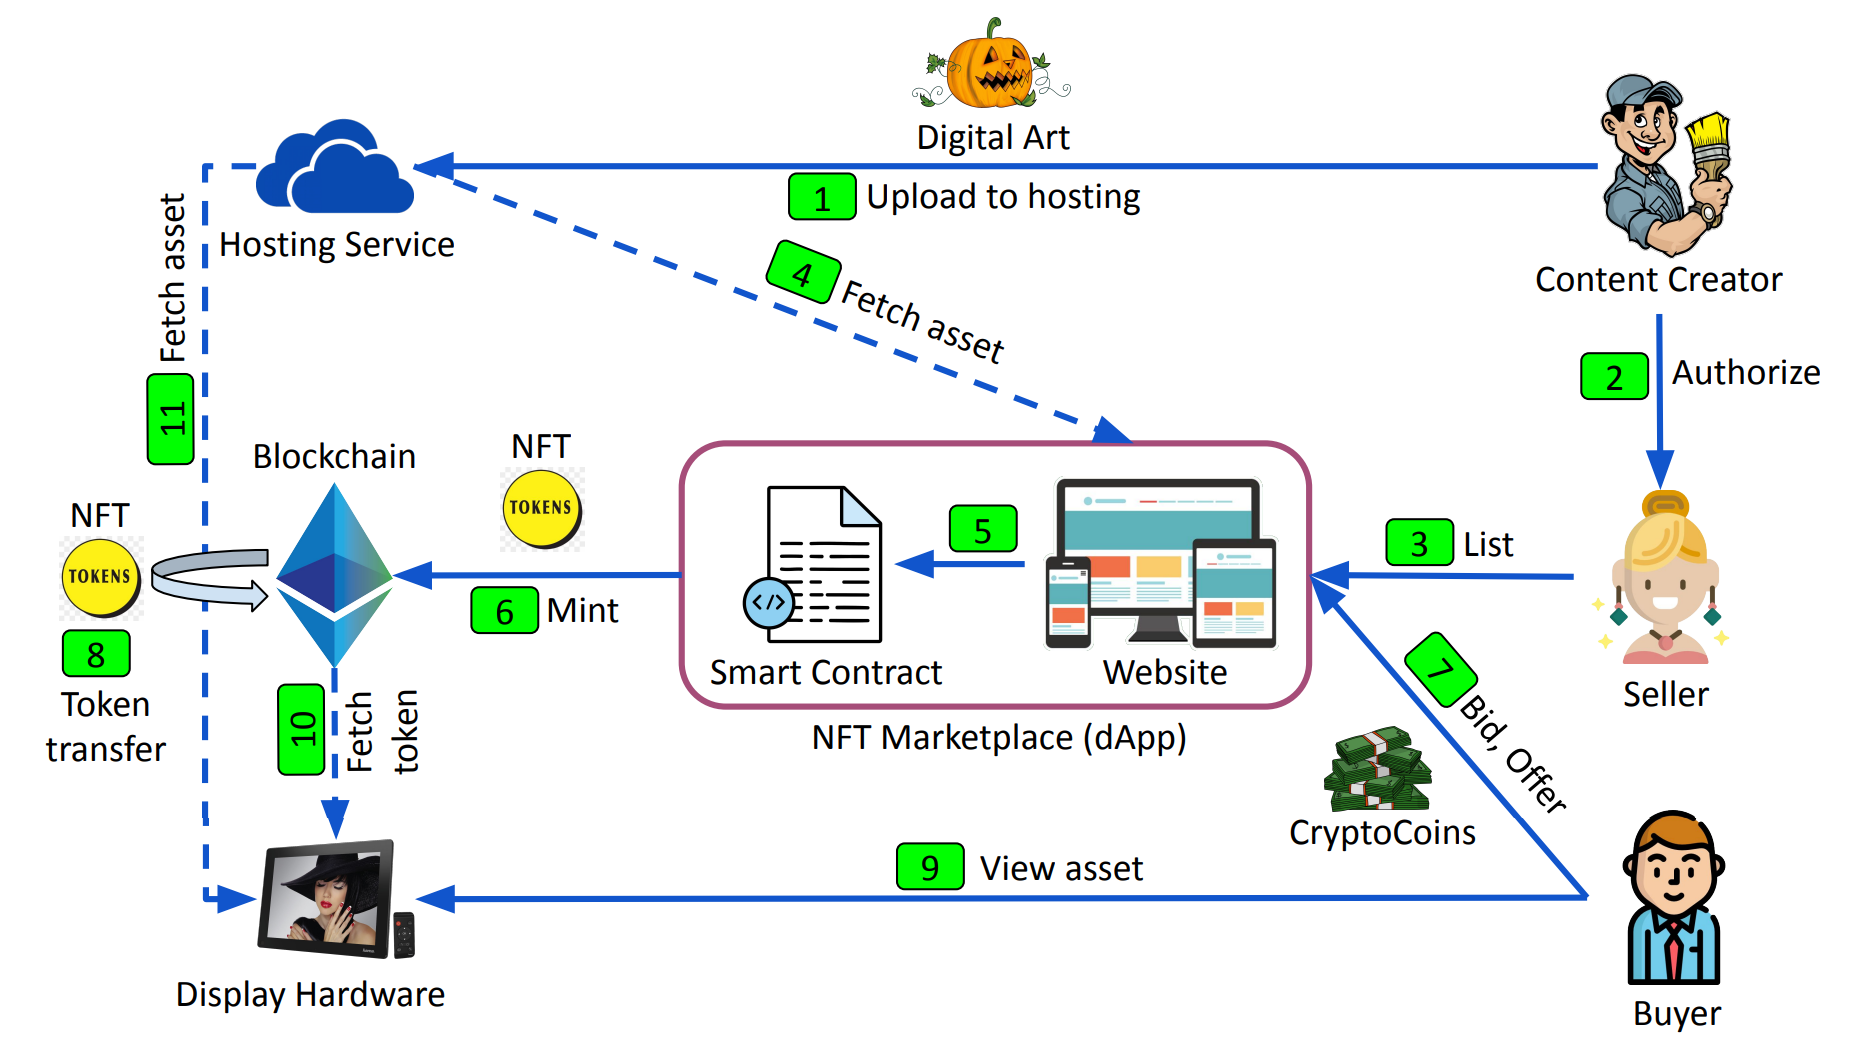
\includegraphics[width=1\textwidth]{Figure/Network Flow.jpg}
\caption{\label{fig:Network}Non-Fungible Dealing Network Flow}
\end{figure*}

As Figure.\ref{fig:Network} shows, the NFT economy is visualized as several building blocks. Among them, let’s specifically focus on the Users part due to their importance. 
The users in the NFT ecosystem could be divided into three categories: creator, buyer, and seller.To begin with, the artist (creators) create digital artwork and upload it to hosting services (an external entity) to make the art publicly available(1). When trading is going to be activated, some creators are not technical enough to mint the NFT for their art and put it on the blockchain. Therefore, they authorize sellers(2) to do this for them(6) and list it on marketplaces. Sometimes, a content creator is also playing the role of the seller. Once listed on a marketplace(3), buyers are able to buy the creatives at a listed price, request offers, or place bids(7). If their offer is accepted or they win an auction, the NFT is transferred(8) by invoking the transferFrom() API to the buyer to reflect the change in ownership~\cite{das2022understanding}.

%-------------------------------------------------------------------------------
\section{Issuance of NFT Projects}
%-------------------------------------------------------------------------------

To better understand the behaviours of users and the factors that can affect NFT prices, we need to first be clear about how NFTs are generated and marketed. The process of issuing an NFT consists of the following steps \cite{how2makenfts}.

\subsection{Pick the Item}
First, we need to determine what unique digital asset we want to turn into an NFT. it can be anything, such as a painting, picture, music, video game, meme, GIF, or even a tweet. An NFT is a unique digital item that has only one owner. This rarity gives NFTs value. However, we must ensure that we own the intellectual property of the item. Creating an NFT for a digital asset that has no intellectual property ownership may lead to legal disputes.

\subsection{Choose Blockchain}
Once we have chosen our unique digital asset, it is now time to begin the process of casting it as an NFT. This starts with determining which blockchain technology we intend to use for NFT. The most popular among NFT artists and creators is Ethereum. Other popular choices include Tezos, Polkadot, Cosmos, and Binance Smart Chain.

\subsection{Set Up Digital Wallet}
Next, we need to set up a digital wallet to create the NFT, as we will need some cryptocurrency to fund our initial investment. The wallet will provide us with access to our digital assets. Top NFT wallets include Metamask, Math Wallet, AlphaWallet, Trust Wallet, and Coinbase Wallet \cite{how2makenfts}.
Once we set up our digital wallet, we want to buy some cryptocurrency. Most NFT platforms accept ethereum, the cryptocurrency of the ethereum blockchain platform.

\subsection{Select NFT marketplace}
Once we have a digital wallet and some cryptocurrency, it's time to start creating (and hopefully selling) our NFT. For that, we need to choose an NFT marketplace. Some of the top NFT marketplaces include OpenSea, Axie Marketplace, Larva Labs/CryptoPunks, NBA Top Shot Marketplace, Rarible, SuperRare, Foundation, Nifty Gateway, Mintable , and ThetaDrop.

Different NFT marketplaces are good fit for different kinds of NFT. For example, Axie Marketplace is the online store for the top NFT game Axie Infinity. Meanwhile, NBA Top Shot is a basketball-focused marketplace. It's also important to note that some marketplaces require their own cryptocurrency. For example, Rarible requires Rarible.
OpenSea is usually a good place to start, as it is the leader in NFT sales. In August 2021 alone, this NFT marketplace sold \$3.4 billion worth of NFT \cite{how2makenfts}.

After selecting your NFT marketplace, we need to connect it to our digital wallet. That will allow us to pay the necessary fees to mint our NFT and hold any sales proceeds.

\subsection{Upload the Item}
We are now finally ready to mint our NFT. The NFT marketplace of choice should have a step-by-step guide to uploading digital files to their platform. This process will allow us to turn our digital files (PNG, GIF, MP3 or other file types) into saleable NFTs.

\subsection{Set up the Sales Process}
The final stage of the NFT minting process is to decide how we want to monetize NFT. Depending on the platform, there are three options.

1. Sell at a fixed price. By setting a fixed price, the first person willing to meet that price can buy your NFT.

2. Set up a timed auction. A timed auction will give those interested in our NFTs a time limit to submit their final bid.

3. Start an unlimited auction. Unlimited auctions do not set a time limit. Instead, we have control and can end the auction at any time.

When setting up an auction, we need to determine the minimum price. It is important to keep the fees in mind when setting the minimum price because if we set the price too low, we may lose money.

Unfortunately, the fees for casting and selling NFT's can be expensive and confusing. Depending on the platform and pricing, they may charge listing fees, NFT minting fees, sales commissions, and transaction fees for transferring money from the buyer's wallet to ours \cite{how2makenfts}. Fees can also fluctuate depending on the volatility of cryptocurrency pricing. Because of this, it's important to pay close attention to the fees we have to pay for minting and selling NFTs to make sure they are worth it.


%-------------------------------------------------------------------------------
\section{NFTs Users and Market Analysis}
%-------------------------------------------------------------------------------

NFTs have exploded in 2021, with a rapid increase in the amount of NFTs being created, bought, and sold, and with tens of billions of dollars worth of cryptocurrency invested in the asset class this year. According to Chain analysis, in 2021, “users have sent at least \$ 44.2 billion worth of cryptocurrency to ERC-721 and ERC-1155 contracts, the two types of Ethereum smart contracts associated with NFT marketplaces and collections ~\cite{tumblr_team_2022}.” But who’s buying NFTs and what are their motivations? What platforms are they using? The users in the NFT ecosystem belong to one of three categories: content creator, seller, and buyer~\cite{das2022understanding}. In this section, the above three categories, content creator, buyer, and seller will be discussed; a brief analysis of the NFTs market trends will also be included. 


\subsection{Content Creator}
The content creators create digital content of an NFT and upload it to hosting services to make their artworks available in public. Some creators are not technical enough to turn their art into an NFT, so they authorize sellers to make their art into NFTs and offer them on marketplaces. Sometimes, a content creator is also taking the role of the seller~\cite{das2022understanding}. The growth of NFTs can help content creators be rewarded fairly for their works by certificating the ownership of their works on the internet~\cite{isak_2021}.


\subsection{NFTs Buyers}
The NFTs buyers refer to those who pay to buy NFTs. According to the article, NFT Audience Insights: Who’s Buying NFTs and Why, there are more than 95,581 active wallets on nonfungible.com, the world’s largest NFTs data resource, by the end of October 2021~\cite{colormatics}. The article analyzes the top states and cities in the U.S. where people are interested in NFTs, pointing out that the top 5 cities that had the highest keyword search for NFTs were all in California and the article identifies that all these locations can be categorized as geographic tech hubs, where the tech industry flourishes. Age, gender, and income surveys have been conducted to NFTs buyers, concluding that “young, tech-savvy audiences with disposable income” are the ones that are most active in the NFTs buyer market~\cite{colormatics}. The motivation of buyers includes making profits, wanting to collect NFTs, valuing the scarcity of NFTs, and supporting their favorite artists~\cite{colormatics}. 

\subsection{NFTs Seller}
NFTs sellers include those who are authorized to make content creators’ work into NFTs and sell them. Sometimes, the NFTs sellers are just the content creator~\cite{das2022understanding}.


\subsection{NFTs Market Trends}
According to Chain analysis, the following Figure.\ref{fig:week} shows the weekly total cryptocurrency value and average value per transaction sent to NFT platforms in 2021. The figure shows that NFTs as an asset category is gaining value and attracting new users~\cite{tumblr_team_2022}. NFTs retail level transactions are transactions below \$ 10,000 worth of cryptocurrency, collector-sized transactions are transactions between \$ 10,000 and \$ 100,000 worth of cryptocurrency and Institutional transactions are transactions above \$ 100,000 worth of cryptocurrency~\cite{tumblr_team_2022}. Although as shown in Figure.\ref{fig:transactions}, the vast majority of NFTs transactions are at the retail level, larger NFTs transactions are becoming more and more common. If we look at the transaction volume instead of the number of transactions, as shown in Figure.\ref{fig:transactions volume}, NFTs collector-sized and institutional-sized transactions play a much more important role~\cite{tumblr_team_2022}.

\begin{figure}[htbp]
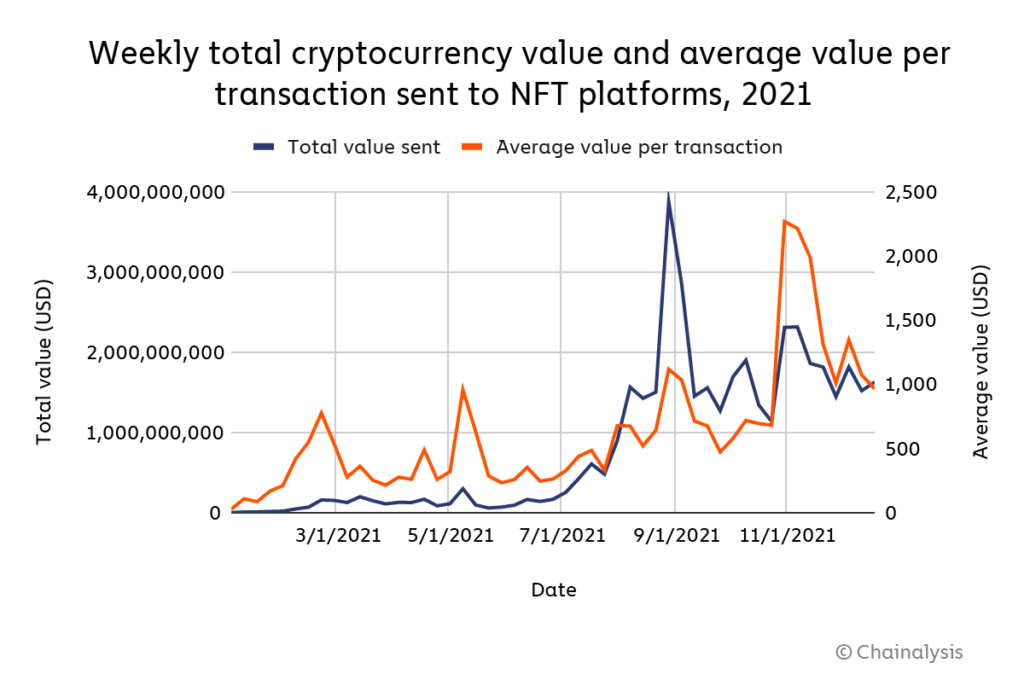
\includegraphics[width=0.5\textwidth]{Figure/The weekly total cryptocurrency value.png}
\caption{The weekly total cryptocurrency value and average value per transaction sent to NFT platforms in 2021.~\cite{tumblr_team_2022}}
\label{fig:week}
\end{figure}

\begin{figure}[htbp]
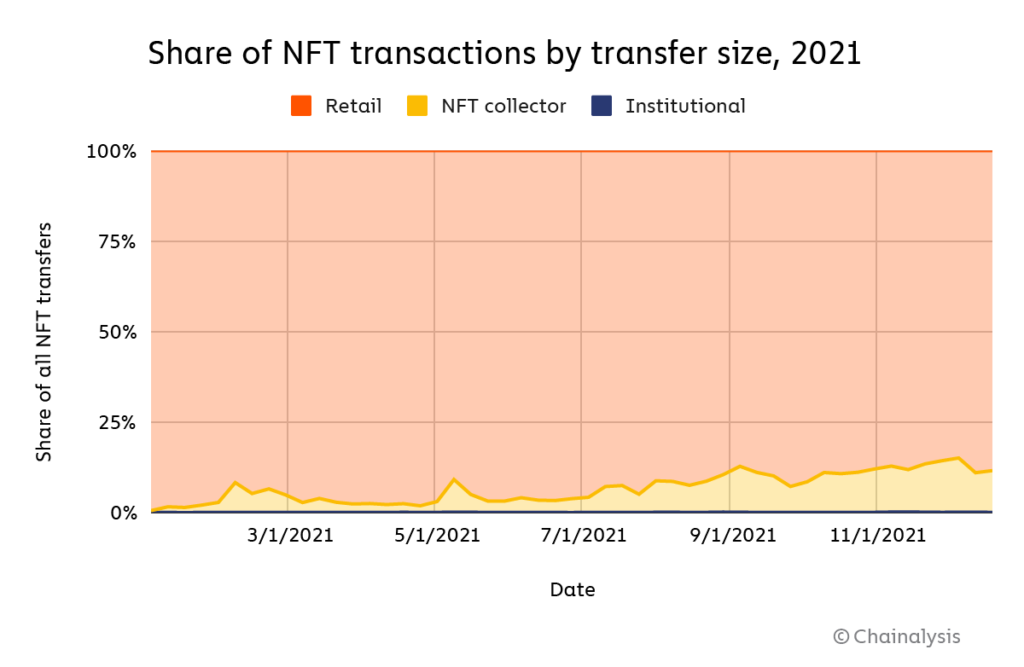
\includegraphics[width=0.5\textwidth]{Figure/transactions.png}
\caption{The share of NFTs transactions by transfer size in 2021.~\cite{tumblr_team_2022}}
\label{fig:transactions}
\end{figure}

\begin{figure}[htbp]
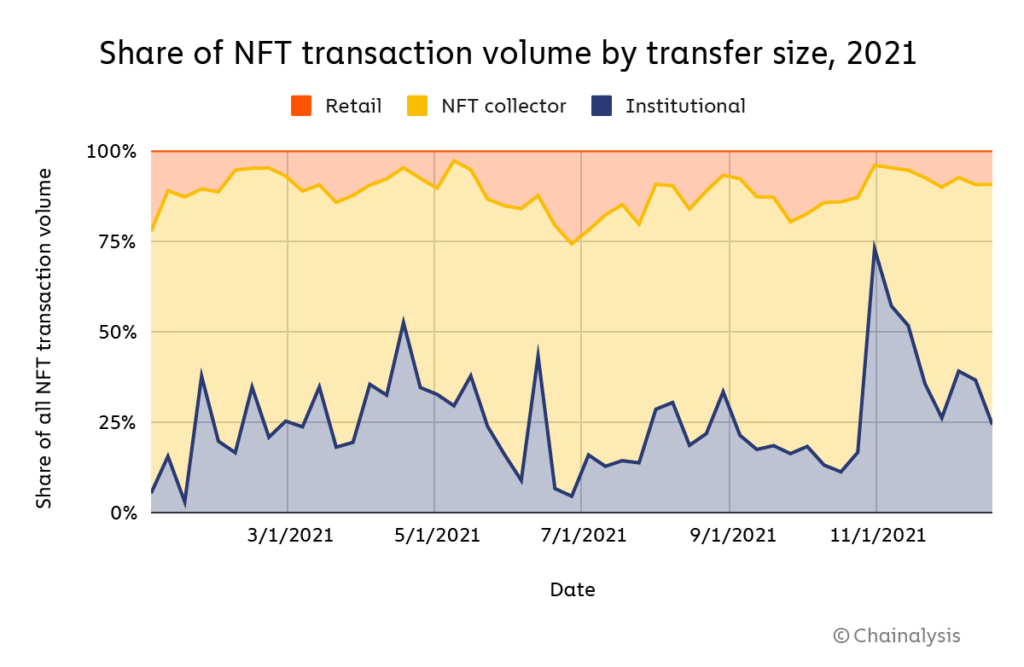
\includegraphics[width=0.5\textwidth]{Figure/transactions volume.png}
\caption{The share of NFT transaction volume by transfer size in 2021.~\cite{tumblr_team_2022}}
\label{fig:transactions volume}
\end{figure}

%-------------------------------------------------------------------------------
\section{Factors that Affect NFT Prices and Project Success.}
%-------------------------------------------------------------------------------

Since the exponential growth of NFT markets, more and more investors start to invest in NFT as part of their asset component. After exploring the basic idea of NFT, issuance mechanism of NFT project, NFTs users and market analysis, it is time to investigate the factors that affect NFT prices and project success. Here, we are going to explore six factors (the digital abundance of NFTs, NFT’s category, the degree and PageRank centrality of the buyer and seller in the networks of NFT trades, NFT’s visual features, the past median price of primary and secondary sales within the collection) that may affect NFT’s prices and project success with a focus on the NFT’s category and past price.


\subsection{The digital abundance of NFTs}

Like real word object, the price of NFT is also highly negative correlated to the digital abundance of NFTs.
"Empirical studies aiming at characterizing properties of the market have focused on a limited number of NFT collections, such as, CryptoKitties17,18, Cryptopunks, and Axie19, or on a single NFT market, such as, Decentraland or SuperRare. These analyses revealed that the digital abundance of NFTs in digital games has led to a substantial decrease of their value, and that, even if NFT prices are driven by the prices of cryptocurrencies, the NFT market could be prone to speculation."\cite{nadini2021mapping}.

\subsection{NFTs Catagory}

NFTs can also be divided into different categories. Most NFTs can be divided in to six categories: Art, Collectible, Game, Metaverse, Other, and Utility.
Each category contribute differently to the whole NFT market. Before the end of 2018, the NFT market mostly include Art category. Later, other category start to grow. By the end of July 2020, Games, Metaverse and Art contributed most of the NFTs market. Hence, releasing a NFT that fall into a growing category may be a great idea to ensure the NFT's value. Besides the total number of NFTs in the market, we also need to consider the number of transactions of each NFT's category. "Since July 2020, the most exchanged NFTs belong to the categories Games and Collectible, which account for 44 percent and 38 percent of transactions. Instead, only 10 percent of transactions are related to NFTs categorized as Art." \cite{nadini2021mapping}. The difference between the volume and number of transactions reveals the price of certain category. For example, the volume of art category is high, but the number of transactions of art is low. This may imply that the price of Art category is higher. For the price distribution of different category, we noticed that "NFTs categorized as Art, Metaverse, and Utility reached higher prices compared to other categories, with the top 1 percent of assets having average sale price higher than 6290, 9485, and 12,756 dollars respectively.\cite{nadini2021mapping}" This also shows that the NFTs under the Art category may have a higher value compare to the NFTs in other category.

\subsection{the degree and PageRank centrality of the buyer and seller}

In real word, many brand invite celebrities to make advertisement of their product to increase the popularity and potential price of their product. This is also true in the NFTs market. After the exponential growth of the NFTs market, many celebrities enter the NFT market by making NFTs for themselves. Many sport stars earn millions of dollars through making their own NFTs. If the NFTs already have enough popularity in the real word, the value of NFT will also be higher."Several other record sales followed10,11: three Cryptopunks—a collection of 10,000 unique automatically generated digital characters—were sold at \$11.8, \$7.6, and \$7.6 million dollars, respectively; the first tweet was sold at \$2.9 million dollars; and the Auction Winner Picks Name, an NFT with music video and dance track, sold at \$1.33 million dollars."\cite{nadini2021mapping}. From the data of those expensive celebrities NFTs and NFTs with some meaning behind it, we can conclude that NFTs valued by experts are more general more successful.  

\subsection{NFT’s visual features}

Through the research, "These two families of features have the largest compound effect in the Art category; in the secondary sale price prediction, centrality features boost the predictive power of visual features by more than 50\%"\cite{nadini2021mapping}, we can see that there is also a relationship between visual features and the NFTs' price. However, because there is a relative large difference between the visual features between each NFTs collection, the comparison between collection based on visual features may not be accurate.

\subsection{The past median price of primary and secondary sales}

NFT's price have a strong correlation between the price of NFT's previously sold within the same collection. "Te median sale price of NFTs in the collection predicts more than half of the variance of price of future primary and secondary sales. Te prediction is more accurate when the median of the past sale price is calculated over a recent time window preceding the primary sale"\cite{nadini2021mapping}. This also match the object in real word, the more the primary sale an object is, the higher the secondary sale we can expect. 

\subsection{Bull and Bear Market}
Like traditional stock market, The NFT market also have a clear bull and bear market phenomena over the year. From a bull to a bear market, the performance for different crypto currency is different. "Ethereum and Litecoin appear to become more illiquid, as opposed to Bitcoin, which appears to become more liquid."\cite{Bull_Bear}. Hence, to increase the possibility of a success project, it is better to release the project during the bull market since there is more liquid in the NFT market.

%-------------------------------------------------------------------------------
\bibliographystyle{plain}
\bibliography{Cite}

%%%%%%%%%%%%%%%%%%%%%%%%%%%%%%%%%%%%%%%%%%%%%%%%%%%%%%%%%%%%%%%%%%%%%%%%%%%%%%%%
\end{document}
%%%%%%%%%%%%%%%%%%%%%%%%%%%%%%%%%%%%%%%%%%%%%%%%%%%%%%%%%%%%%%%%%%%%%%%%%%%%%%%%

%%  LocalWords:  endnotes includegraphics fread ptr nobj noindent
%%  LocalWords:  pdflatex acks